%         Created on  11-JANUARY-1996 by Phillip Gutierrez
%-------------------------------------------------------------------
\tolerance 1000
%\documentclass[portrait]{seminar}
\documentclass{seminar}
%
\usepackage{graphicx}
\usepackage{amsmath}
\usepackage{latexsym}
\usepackage{amssymb}
%\usepackage[dvips]{color}
\usepackage[dvips]{pstcol}
\usepackage{semcolor}
%\usepackage{colordvi}
\usepackage{blackdvi}

\usepackage{fancybox}
%\usepackage{fancyhdr}
%\textwidth 6.5in
%\textheight 8.5in
\textwidth 8.5in
\textheight 6.5in
\topmargin 0in
\oddsidemargin 0in
\evensidemargin 0in
%\parskip 1.5ex
\baselineskip 3.0ex
%\usepackage{fancyheadings}
\slidesmag{4}
%\input my_colors

\newpagestyle{myslide}{\Gray{\sl P.~Gutierrez \hfil \hfil May 13, 2004}}
                      {\Gray{\sl D\O \hfil Slide-\thepage
                                                      \hfil Mixing Meeting}}
\newpagestyle{myempty}{}{}
\Gray{
\pagestyle{myslide}
\slideframe{oval}}
%%
%\input d0_style.tex
% \newcommand{\black}{\color{black}}
% \newcommand{\red}{\color{red}}
% \newcommand{\magenta}{\color{magenta}}
% \newcommand{\green}{\color{green}}
% \newcommand{\blue}{\color{blue}}
% \newcommand{\cyan}{\color{cyan}}
% \newcommand{\yellow}{\color{yellow}}
\newcommand{\mpg}{\color [rgb]{.5,.5,.5}}
%
\newcommand{\clraa}{\color [rgb]{.7,0,.1}}
\newcommand{\clrc}{\color [rgb]{.1,1,1}}
\newcommand{\clrb}{\color [rgb]{.4,0,1}}
\newcommand{\clrn}{\color [rgb]{.4,0,.3}}
\newcommand{\clrm}{\color [rgb]{1,0,.3}}
%%
\renewcommand{\labelitemi}{$\blacksquare$}
\renewcommand{\labelitemiv}{$\bullet$}
\renewcommand{\labelitemiii}{$\blacktriangle$}
\renewcommand{\labelitemii}{$\blacklozenge$}
\renewcommand{\labelitemi}{$\Box$}
\renewcommand{\labelitemiv}{$\triangleright$}
\renewcommand{\labelitemiii}{$\circ$}
\renewcommand{\labelitemii}{$\Diamond$}
%
\newcommand{\hdr}[1]{\begin{center}{\WildStrawberry{\Large\bf #1}}\end{center}}
%
%%%%%%%%%%%
%
\newcommand{\hdra}[1]{
            \begin{center}
            \Ovalbox{\noindent
            \makebox[4.8in][c]{
            \makebox[.51in][c]{\includegraphics[width=.5in]{figs/d0}}
            \hfill
            \raisebox{2ex}{
            \parbox[c]{3.2in}{\Large\bf \red #1}}
            \hfill
            \makebox[.51in][c]{\includegraphics[width=.5in]{figs/cdf}}}}
            \end{center}
            \vspace{2mm}\hrule\vspace{.5mm}\hrule\vspace{2mm}}
%
%%%%%%%%%%%%
%
\newcommand{\hdrps}[1]{
            \begin{center}
            \psframebox[framearc=0.4, fillstyle=solid, fillcolor=yellow]{\noindent
            \makebox[4.8in][c]{
            \includegraphics[width=.5in]{figs/d0}
            \hfill
            \raisebox{2ex}{
            \parbox[c]{3.4in}{\begin{center}\Large\bf \RedOrange{#1}\end{center}}}
            \hfill
            \includegraphics[width=.5in]{figs/cdf}}}
            \end{center}
            %\vspace{2mm}\hrule\vspace{.5mm}\hrule\vspace{2mm}
            }
%
%%%%%%%%%%%
%
\newcommand{\hdrb}[1]{
            \begin{center}
            \Ovalbox{\noindent
            \makebox[4.8in][c]{
            \includegraphics[width=.7in]{d0_logo}
            \hfill
            \raisebox{2ex}{
            \parbox[c]{3.4in}{\begin{center}\Large\bf \RedOrange{#1}\end{center}}}
            \hfill
            \includegraphics[width=.4in]{ou}}}
            \end{center}
            %\vspace{2mm}\hrule\vspace{.5mm}\hrule\vspace{2mm}
            }
%
%%%%%%%%%%%%
%
\newcommand{\Lt}{\ensuremath{\int\mathcal{L}\, dt}}
\newcommand{\ee}{\ensuremath{e^+e^-}}
%%%%%%
%\newenvironment{citemize}[2][black]{\begin{itemize}\textcolor{#1}{#2}}
%                                  {\end{itemize}}
%%%%%%
%\input my_macs
%\input colordvi
%\definecolor{iMidnightBlue}{cmyk}{0.98, 0.13, 0, 0.4}
\begin{document}
%
%\pagestyle{myslide}
%
% Some counters
%
%\newcounter{my1}
%\newcounter{my2}
%\newcounter{my3}
%\newcounter{my4}
%\newcommand{\my1_inc}{\setcounter{my1}{\value{enumi}}}
%\newcommand{\ST_CNTR_1}{setcounter{my1}{\value{enumi}} }
%
%%%%%%%%%
%
\thispagestyle{myempty}
\begin{slide}
%\vfill
\begin{center}%\textcolor{red}
{\huge {\bf \WildStrawberry{Combining Flavor Taggers}\\}}
\vspace{1cm}
%\textcolor{red}
{\Large\it \RoyalBlue{How Best to Combine the Taggers?}\\}
\end{center}
\vspace{1.5cm}
\begin{center}
{\it \Plum{P. Gutierrez---University of Oklahoma}\\}
\end{center}
%\vfill
\end{slide}
%
%%%%%%%%%
%
\slideframe{oval}
\centerslidesfalse
%
%%%%%%%%%
%
\begin{slide}
\hdr{Where We Stand}
\begin{itemize}
  \item \BlueViolet{At present we have three taggers}
  \begin{itemize}
    \item \WildStrawberry{$\text{SLT}\equiv\text{Single Lepton Tag}$}
    \item \WildStrawberry{$\text{STT}\equiv\text{Same Side Tag}$}
    \item \WildStrawberry{$\text{JETQ}\equiv\text{Jet Charge}$}
  \end{itemize}
  \item \BlueViolet{The questions we wish to answer is how best to
                    combine the taggers to minimize the error
                    on $\Delta m$}
\end{itemize}
\end{slide}
%
%%%%%%%%%
%
\begin{slide}
\hdr{How to Combine Tagger Significance}
\begin{itemize}
  \item \BlueViolet{Reminder, we want to maximize 
         is \Magenta{$\epsilon D^2$} or minimize
                   the error on \Magenta{$\Delta m$}.}
		   \begin{align*}\Red{
		     &\sigma \propto \frac{1}{\sqrt{N\epsilon D^2}}}\qquad
		     \text{\RoyalBlue{or}} \qquad \Red{S\equiv\text{Significance}
		     \propto \sqrt{N\epsilon D^2}}\\\Magenta{
		     &\epsilon = \frac{\text{tagged}}{\text{total sample}}\qquad
		      D= \frac{\text{Correct tags} - \text{Wrong tags}}
		              {\text{Total tagged}}}
		   \end{align*}
  \item \BlueViolet{Recall, \Magenta{error} for 
         \Magenta{$n$ independent measurements} is given by}
	\begin{displaymath}\Red{
	  \frac{1}{\sigma^2} =\sum_i^n\frac{1}{\sigma_i^2}\propto
	  S^2}
	\end{displaymath}
  \item \BlueViolet{Therefore, if \Magenta{$n$ taggers are 
         independently used,}
        then} $\Red{S^2 \propto\sum_i^n \epsilon_i D^2_i}$
\end{itemize}
%
%%%%%%%%%
%
\end{slide}
%
%%%%%%%%%
%
\begin{slide}
\hdr{Approach to study}
\begin{itemize}
  \item \BlueViolet{Use toy Monte Carlo to generate a sample of events}
  \item \BlueViolet{Start with \Magenta{$\epsilon$} \& 
        \Magenta{$D$} given by Christos}
\end{itemize}
  \vfill
  \begin{center}
    \begin{tabular}{|c|r|r|}\hline
      Tag &
      \multicolumn{1}{|c}{$\epsilon$} &\multicolumn{1}{|c|}{$D$}\\
      \hline\hline
      SLT & \hspace{1cm} 5.2\% & \hspace{1cm}42.0\%\\
      SST & 83.3\% & 14.4\% \\
      JETQ & 51.1\% & 13.7\% \\\hline
    \end{tabular}
  \end{center}
  \vfill
\end{slide}
%
%%%%%%%%%
%
\begin{slide}
\hdr{Taggers}
  \begin{itemize}
    \item \BlueViolet{Considered 3 tagging methods}
    \begin{itemize}
      \item \RoyalBlue{1 measurement use tag with largest dilution}
    \end{itemize}
  \end{itemize}
%
    \begin{center}{\footnotesize
    \begin{tabular}{|r|r|r|}
    \hline
     \multicolumn{1}{|c}{$\epsilon$}&\multicolumn{1}{|c}{$D$}
     &\multicolumn{1}{|c|}{\Red{$\epsilon D^2$}}\\ \hline\hline
      \hspace{10mm}92.2\% & \hspace{10mm}15.9\% 
              & \hspace{10mm}\Red{2.3\%}\\\hline
    \end{tabular}}
    \end{center}\vspace{2mm}
  \begin{itemize}
    \item[]
    \begin{itemize}
      \item \RoyalBlue{3 independent measurements}
      \begin{itemize}
        \item $\WildStrawberry{\text{tag1} = \text{SLT}}$
	\item $\WildStrawberry{\text{tag2} = \text{SST if not tagged by SLT}}$
	\item $\WildStrawberry{\text{tag3} = \text{JETQ
	      if not tagged by either SLT or SST}}$
      \end{itemize}
    \end{itemize}
  \end{itemize}
\begin{center}
  {\footnotesize
  \begin{tabular}{|c|r|r|r|}
  \hline
  Tag & \multicolumn{1}{|c}{$\epsilon$}&\multicolumn{1}{|c}{$D$}
  &\multicolumn{1}{|c|}{\Red{$\epsilon D^2$}}\\ \hline\hline
  tag1 & \hspace{10mm}5.2\% & \hspace{10mm}42\% & \hspace{10mm}0.91\%\\
  tag2 & 79.0\% & 14.4\% & 1.65\%\\
  tag3 & 8.1\% & 13.6\% & 0.15\%\\
  \hline
  Sum & & & \Red{2.71\%}\\\hline
  \end{tabular}}
\end{center}
\end{slide}
%
%%%%%%%%%
%
\begin{slide}
\hdr{Taggers---{\em cont.}}
  \begin{itemize}
    \item[]
    \begin{itemize}
      \item \RoyalBlue{Make five independent measurements}
      \begin{enumerate} 
        \item \WildStrawberry{$\text{tag1}=\text{SLT}$;}
	      \Thistle{Exclude these from remaining tags}
	\item \WildStrawberry{if $\text{SST}=\text{JETQ}$ 
	       then $\text{tag2} = \text{SST}$}
	\item \WildStrawberry{if $\text{SST}\ne\text{JETQ}$
	      then $\text{tag3} = \text{SST}$}
	\item \WildStrawberry{if only SST $\text{tag4}=\text{SST}$}
	\item \WildStrawberry{if only JETQ $\text{tag5}=\text{JETQ}$}
      \end{enumerate}
    \end{itemize}
  \end{itemize}
\begin{center}
  {\footnotesize
  \begin{tabular}{|c|r|r|r|}
  \hline
  Tag & \multicolumn{1}{|c}{$\epsilon$}&\multicolumn{1}{|c}{$D$}
  &\multicolumn{1}{|c|}{\Red{$\epsilon D^2$}}\\ \hline\hline
  tag1 & \hspace{10mm}5.2\% & \hspace{10mm}42\% & \hspace{10mm}0.91\%\\
  tag2 & 20.6\% & 27.8\% & 1.59\%\\
  tag3 & 19.7\% & -0.6\% & 0.00\%\\
  tag4 & 38.7\% & 14.4\% & 0.80\%\\
  tag5 & 8.1\% & 13.6\% & 0.15\%\\
  \hline
  Sum & & & \Red{3.45\%}\\\hline
  \end{tabular}}
\end{center}
\
\end{slide}
%
%%%%%%%%%
%
\begin{slide}
\hdr{A Sanity Check}
\begin{itemize}
  \item \BlueViolet{Generated 10K events with previously
        given
        \Magenta{$\epsilon$} and \Magenta{$D$}}
  \item \BlueViolet{Fit lifetime distributions
         using an unbinned Likelihood function}
  \begin{itemize}
    \item \RoyalBlue{Fit for Lifetime, Resolution, 
          $\Delta m$, and Mistag Rate}
  \end{itemize}
\end{itemize}
\begin{multline*}\Red{
  L^{\text{U/M}}
    =(1-\RoyalBlue{\alpha})\int
     e^{-(t-t')/2\RoyalBlue{\sigma}^2} e^{-t/\RoyalBlue{\tau}}
                      [1 \pm \cos(\RoyalBlue{\Delta m})]\, dt'+\\
       \RoyalBlue{\alpha}
       \int e^{-(t-t')/2\RoyalBlue{\sigma}^2}
                      e^{-t/\RoyalBlue{\tau}}
                      [1 \mp \cos(\RoyalBlue{\Delta m})]\, dt'}
\end{multline*}
\begin{itemize}
  \item \BlueViolet{Initial parameters}
  \begin{itemize}\WildStrawberry{
    \item $\tau=1.5$ ps
    \item $\sigma=.5$ ps
    \item $\Delta m=0.51$ ps$^{-1}$
    \item Dilutions as given earlier}
  \end{itemize}
\end{itemize}
\end{slide}
%
%%%%%%%%%
%
\begin{slide}
\hdr{Examples of Fits}
\begin{itemize}
  \item \BlueViolet{Lifetime distribution of mixed and unmixed sample
        for SLT and (SLT*SST*JETQ) Combined tags}
\end{itemize}
\begin{center}
\includegraphics[width=.60\textwidth]{tag1_10K.eps}
\vfill
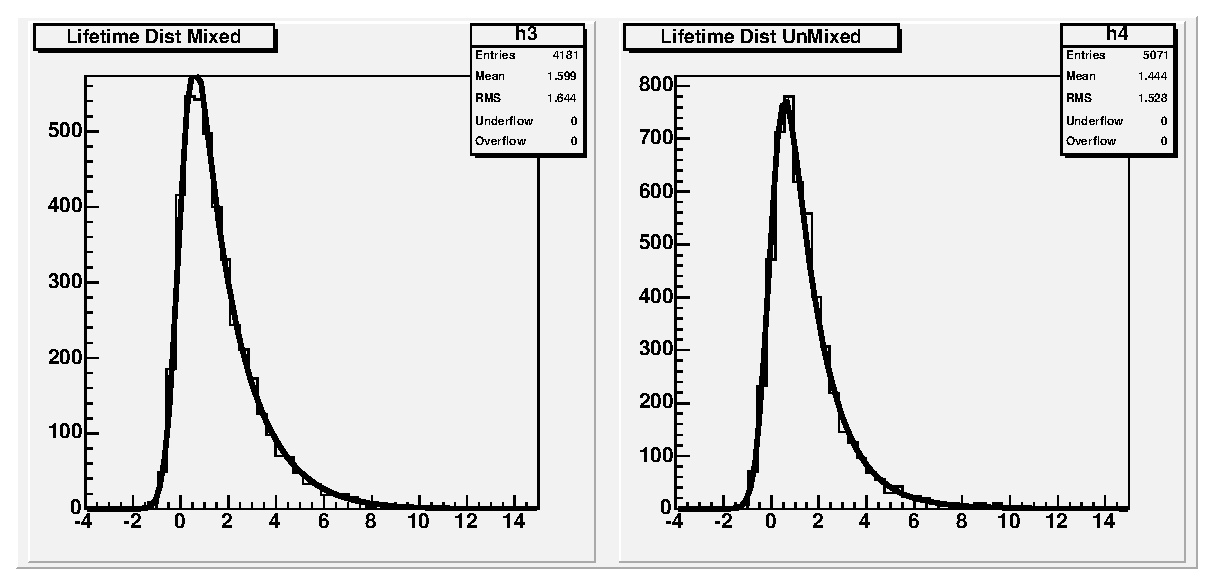
\includegraphics[width=.60\textwidth]{tag8_10K.eps}
\vfill
\end{center}
\end{slide}
%
%%%%%%%%%
%
\begin{slide}
\hdr{Comparison of errors and $\epsilon D^2$}
\begin{itemize}	
  \item \BlueViolet{Compare errors of $\Delta m$ \Red{for single measurement
        $\epsilon D^2=2.3\%$} and combine \Red{5 measurments
	$\epsilon D^2=3.45\%$}}
\end{itemize}
\begin{minipage}[t]{.47\textwidth}
\begin{center}
  Errors\\\vspace{2mm}{\footnotesize
  \begin{tabular}{|c|r|r|}\hline
  Tag & \multicolumn{1}{c}{\Blue{Error (ps$^{-1}$)}} 
      &\multicolumn{1}{|c|}{\Red{$\epsilon D^2$}}\\
  \hline\hline
  Single Tag & \Blue{0.051} & \Red{0.023}\\\hline
   & & \\
  1 & 0.0665 & 0.91\%\\
  2 & 0.0623 & 1.59\%\\
  4 & 0.0945 & 0.80\%\\
  5 & 0.1857 & 0.15\%\\\hline
 Total & \Blue{0.0400} & \Red{3.45\%}\\
  \hline
  \end{tabular}}
\end{center}
\end{minipage}
%%
\begin{minipage}[t]{.47\textwidth}{\footnotesize
\begin{center}
   \WildStrawberry{Ratios}
\end{center}
\begin{itemize}\RoyalBlue{
  \item $\Red{\sigma_1/\sigma_5=0.784$}
  \item[]
  \item $\Red{\sqrt{\epsilon_5 D^2_5/
       \epsilon_1 D^2_1}
        =0.824$}
  \item[]
  \item Recalculate \Magenta{$\epsilon$} \& \Magenta{$D$}
        for 10K sample
        \Red{$\sqrt{\epsilon_5 D^2_5/
       \epsilon_1 D^2_1}
        =0.786$}}
\end{itemize}}
\end{minipage}
\end{slide}
%
%%%%%%%%%
%
\begin{slide}
\hdr{Summary and Conclusions}\BlueViolet{
\begin{itemize}
  \item Quantity to maximize is $\epsilon D^2$
  \RoyalBlue{
  \begin{itemize}
    \item The significance is $\propto \sqrt{N\epsilon D^2}$
    \item $\epsilon D^2$ add for combined measurements
  \end{itemize}}
  \item The effect of any new tagger can be easily calculated
        once $\epsilon$ and $D$ are known
  \item Current study shows combining 5(4) taggers yields improvement
        over a single tagger
\end{itemize}}
\end{slide}
%
%%%%%%%%%
%
\end{document}

